\documentclass[12pt, a4paper, oneside]{article}
\usepackage{longtable}
\usepackage[
  a4paper, mag=1000, includefoot,
  left=2.3cm, right=1cm, top=2cm, bottom=2cm, headsep=1cm, footskip=1cm
]{geometry}
\usepackage[T2A]{fontenc}
\usepackage[utf8]{inputenc}
\usepackage[english,russian]{babel}
\ifpdf\usepackage{epstopdf}\fi

\usepackage{listings}
\usepackage[pdftex]{lscape}
\usepackage{array}
\usepackage{multirow}
\usepackage{multicol}
\usepackage{mdwlist}
\usepackage{setspace}
\usepackage{indentfirst}
\usepackage{hyperref}
\usepackage{graphicx}
\usepackage{verbatim}
\usepackage{wrapfig}
\usepackage{booktabs}
\usepackage{pscyr}
\usepackage{mdwlist}

\hypersetup{
    bookmarks=true,   
    unicode=true,          
    pdftitle={Программа Морской бой},    
    pdfauthor={Бабарыкин Денис},     
    pdfsubject={Олимпиадная работа},  
    colorlinks=true,      
    linkcolor=blue,         
    citecolor=green,        
    filecolor=magenta,     
    urlcolor=cyan,
    pdfborder = {0 0 0}          
}

\graphicspath{{images/}}

\renewcommand{\lstlistingname}{Листинг}
\lstset{ %
language=C++,                     % the language of the code
basicstyle=\footnotesize,       % the size of the fonts that are used for the code
numbers=left,                   % where to put the line-numbers
numberstyle=\footnotesize,      % the size of the fonts that are used for the line-numbers
stepnumber=1,                   % the step between two line-numbers. If it's 1, each line 
                                % will be numbered
numbersep=5pt,                  % how far the line-numbers are from the code
backgroundcolor=\color{white},  % choose the background color. You must add \usepackage{color}
showspaces=false,               % show spaces adding particular underscores
showstringspaces=false,         % underline spaces within strings
showtabs=false,                 % show tabs within strings adding particular underscores                
tabsize=2,                      % sets default tabsize to 2 spaces
captionpos=b,                   % sets the caption-position to bottom
breaklines=true,                % sets automatic line breaking
breakatwhitespace=false,        % sets if automatic breaks should only happen at whitespace
escapeinside={\%*}{*)},         % if you want to add a comment within your code
morekeywords={*,...},           % if you want to add more keywords to the set
keywordstyle=\color[rgb]{0,0,1},
commentstyle=\color[rgb]{0.133,0.545,0.133},
stringstyle=\color[rgb]{0.627,0.126,0.941}
}



\begin{document}

\begin{center}
\vspace{10cm}

\textsc{\textbf{ОЛИМПИАДА ШКОЛЬНИКОВ «ШАГ В БУДУЩЕЕ»}}\\[1.4cm]

\textsc{\textbf{НАУЧНО-ОБРАЗОВАТЕЛЬНОЕ СОРЕВНОВАНИЕ «ШАГ В БУДУЩЕЕ, МОСКВА»}}\\[1.7cm]

\begin{flushright}
\setlength{\unitlength}{1cm}
\begin{picture}(6.5,0.7)
\put(0,0){\framebox(5.8,0.7){}}
\end{picture}

\small\textit{регистрационный номер~~~~~~~~~~}
\end{flushright}

~

\vspace{-0.1cm}
{
{\textbf{\normalsize\vspace{-0.4cm} Факультет «Информатика и системы управления»}} \\[0.02cm]
\vspace{+0.1cm}\rule{0.9\linewidth}{0.1mm}
~

~

\vspace{-0.7cm}\small\textit{название факультета}
}

{
\textbf{\normalsize{\vspace{-0.2cm}Кафедра «Программное обеспечение ЭВМ и информационные технологии»}} \\[-0.1cm]
\rule{1\linewidth}{0.1mm}
~

\vspace{-0.65cm}\small\textit{название кафедры ~~~~~~~~~~~~~~~~~} \\[0.4cm]
}
~

{
\textbf{\normalsize{\vspace{-0.2cm}«Сетевая игра ``Морской бой''»}} \\[-0.1cm]
\rule{1\linewidth}{0.1mm} \\[0.2cm]

\rule{1\linewidth}{0.1mm} \\[0.2cm]

\hspace{-5.4cm}\rule{0.7\linewidth}{0.1mm} \\[0.2cm]

~

\vspace{-0.8cm}\small\textit{~~~название работы}

}

~

\vspace{1cm}

\begin{tabular}{p{6cm}p{11cm}}
  \textbf{Автор:} & \textbf{Бабарыкин Денис Сергеевич} \\[-0.3cm]
 
  & \rule{\linewidth}{0.1mm} \\[-0.2cm] 
  & \small\textit{~~~~~~~~~~~~~~~~~~~~~ фамилия, имя, отчество ~~~} \\[0.3cm]
  & \vspace{-0.6cm}\textbf{ГБОУ СОШ №81, 11 класс} \\[-0.3cm]
  & \vspace{-0.6cm}\rule{\linewidth}{0.1mm} \\[-0.2cm] 
  & \vspace{-0.6cm}\small\textit{~~~~~~~ наименование учебного заведения, класс ~~~} \\[0.4cm]
  \textbf{Научный руководитель:} & \textbf{Ковтушенко Александр Петрович} \\[-0.3cm]
 
  & \rule{\linewidth}{0.1mm} \\[-0.2cm] 
  & \small\textit{~~~~~~~~~~~~~~~~~~~~~ фамилия, имя, отчество ~~~} \\[0.3cm]
  & \vspace{-0.6cm}\textbf{МГТУ имени Н. Э. Баумана} \\[-0.3cm]
  & \vspace{-0.6cm}\rule{\linewidth}{0.1mm} \\[-0.2cm] 
  & \vspace{-0.6cm}\small\textit{~~~~~~~~~~~~~~~~~~~~~место работы ~~~} \\[0.4cm]
  & \vspace{-0.6cm}\textbf{к. ф.-м. н., доцент} \\[-0.3cm]
  & \vspace{-0.6cm}\rule{\linewidth}{0.1mm} \\[-0.2cm] 
  & \vspace{-0.6cm}\small\textit{~~~~~~~~~~~~~~~~~~~~~звание, должность ~~~} \\[0.4cm]

\end{tabular}

\vfill

\textbf{Москва -- 2012}
\thispagestyle{empty}
\end{center}

\onehalfspacing
\section*{Аннотация}

В рамках данной работы рассмотрено применение языка программирования C++ в сочетании с библиотекой графического интерфейса Qt в контексте разработки кроссплатформенной сетевой игры ``Морской бой''.  Программа состоит из серверной и клиентской частей.  Многопоточный сервер,  реализованный с использованием низкоуровневых системных вызовов, отвечает за взаимодействие игроков, обмен сообщений между ними,  а также восстановление начатой игровой сессии после сбоя. Программа-клиент имеет интуитивно понятный графический интерфейс с элементами реалистичной графики отображения элементов полей игроков. В рамках проекта разработан и реализован протокол взаимодействия сервера и клиента, включающий как передачу команд игры, так и произвольные сообщения в формате чата.  Во время разработки программы были исследованы паттерны проектирования для комбинации различных стратегий автоматической расстановки кораблей с современными методами машинного обучения на основе искусственных нейронных сетей для выбора хода компьютера. Сделаны выводы о возможностях применения искусственных нейронных сетей для решения подобных задач.

\newpage
\tableofcontents
\newpage
\section*{Введение}
\addcontentsline{toc}{section}{Введение}

Работа посвящена созданию кроссплатформенной программы ``Морской бой''  с помощью языка программирования C++ и библиотеки графического интерфейса Qt. Целью данной работы является разработка программы, поддерживающей игру на одном компьютере, через локальную сеть и через Интернет. В задачу также входит исследование различных алгоритмов по выбору наиболее оптимального удара на основе концепции искусственных нейронных сетей и традиционных методов.

\section*{Актуальность работы}
\addcontentsline{toc}{section}{Актуальность работы}

В современном мире все большее значение приобретают требования к безопасности программного обеспечения. Наиболее безопасным следует считать программы с открытым исходным кодом, потому что об их деятельности можно узнать все непосредственно из исходных текстов. Поэтому изучение технологии кроссплатформенного программирования с использованием графической библиотеки Qt, а также системного программирования с использованием низкоуровневых вызовов представляется весьма важной задачей. В рамках данной работы частично были изучены эти технологии и на их основе реализована сетевая игра ``Морской бой''. 

Компьютерные технологии позволяют анализировать большие массивы данных с целью нахождения закономерностей  и прогнозирования их динамики. Применение искусственных нейронных сетей позволяет строить математические модели, когда зависимость между входными и выходными данными невозможно описать в явном виде. Обладая способностью к обучению и обобщению, нейросети представляются идеальными алгоритмами для имитации игры человека компьютером. Актуальность работы и новизна связаны с оценкой применимости искусственных нейронных сетей для выбора ``человеческого'' хода в игре ``Морской бой''. 

\section{Архитектура и принципы функционирования программы}
\subsection{Структура программы}

Как правило компьютеры и программы, входящие в состав современных информационных систем, не являются равноправными. Некоторые из них владеют ресурсами (файловая система, процессор, принтер, база данных, вычислительный кластер), другие имеют возможность обращаться к этим ресурсам. Компьютер (или программу), управляющий ресурсом, называют сервером этого ресурса (игровой сервер, файл-сервер, сервер базы данных, вычислительный сервер). Клиент и сервер какого-либо ресурса могут находиться как в рамках одной вычислительной системы, так и на различных компьютерах, связанных сетью, при этом эти компьютеры могут быть представлены разными архитектурами и операционными системами, рис. \ref{fig:serverclient}.

Основной принцип технологии ``клиент-сервер'' заключается в разделении функций приложения на три группы:
\begin{enumerate*}
    \item ввод и отображение данных (взаимодействие с пользователем);
    \item прикладные функции, характерные для данной предметной области;
    \item функции управления ресурсами (файловой системой, базой данных и т.д.). 
\end{enumerate*}

Поэтому, в любом приложении выделяются следующие компоненты:
\begin{enumerate*}
    \item компонент представления данных;
    \item прикладной компонент;
    \item компонент управления ресурсом. 
\end{enumerate*}

Связь между компонентами осуществляется по определенным правилам, которые называют ``протокол взаимодействия''. В рамках данной работы был реализован собственный протокол взаимодействия клиента (графического приложения, с которым взаимодействует пользователь) с игровым сервером.

\begin{figure}[t]
\begin{center}
	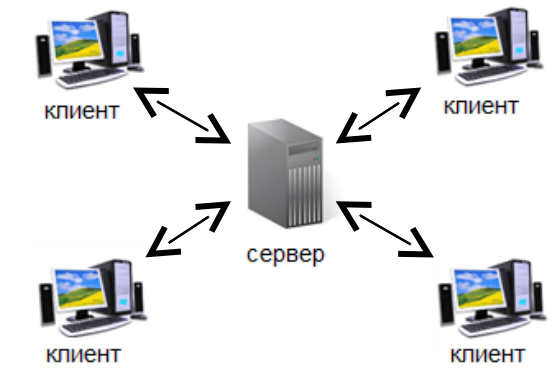
\includegraphics[scale=0.5]{serverclient.png}
	\caption{Схема технологии ``клиент--сервер''.}
	\label{fig:serverclient}
	\vspace{-0.5cm}
\end{center}
\end{figure}

Программа состоит из клиентской и серверной частей. Клиент реализован на языке C++ с применением кроссплатформенной библиотеки Qt в интегрированной среде разработки Qt Creator (Qt Software\texttrademark, Nokia\texttrademark). Программа-клиент обладает дружелюбным пользовательским интерфейсом с 
элементами реалистичной трехмерной графики. Клиент позволяет играть в ``морской бой'' с компьютером, а также по сети с другими игроками через игровой сервер. 

\subsection{Принцип работы клиента}

\begin{figure}[h]
\begin{center}
	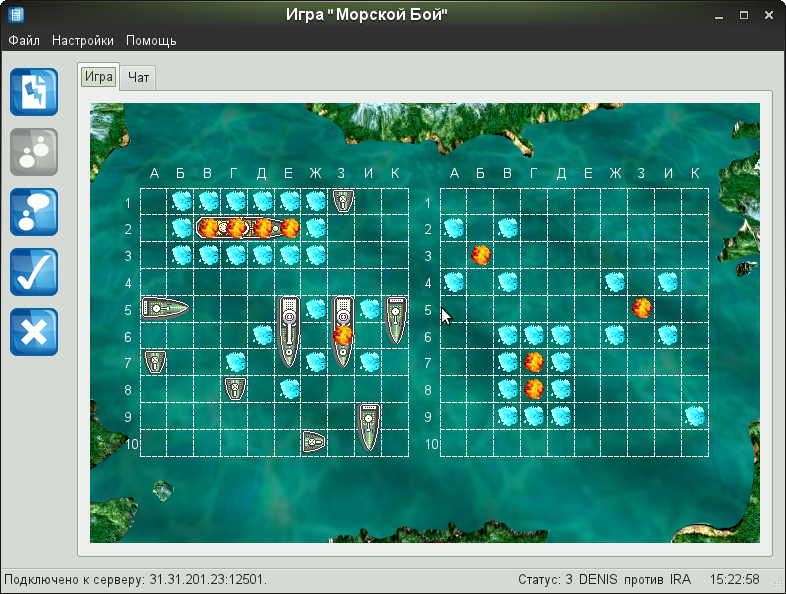
\includegraphics[scale=0.63]{seabattle.png}
	\caption{Скриншот главного окна программы.}
	\label{fig:client}
	\vspace{-0.5cm}
\end{center}
\end{figure}

При работе с программой ``Морской бой'' пользователь может даже не знать о существовании сервера, который обеспечивает взаимодействие клиентов. Скриншот главного окна программы показан на рис. \ref{fig:client}. С программой может играть самый обыкновенный человек, далекий от программирования и сетевых технологий.

Приложение-клиент состоит из игровых полей противников, меню и кнопок управления. Сначала игрок расставляет корабли в специальном диалоге, доступном по кнопке ``Расставить корабли''. Затем он может либо подключиться к игровому серверу, указав его адрес и порт, а также ник -- имя, под которым данный игрок будет виден другим игрокам; либо начать игру с компьютером, выбрав при этом уровень сложности. На сложность влияет тактика расстановки кораблей и наличие в алгоритме игры нейросетевой модели по определению места удара машины.

Если пользователь выбирает сетевой вариант игры, то ему необходимо подобрать себе соперника. Для этого предусмотрена функция отображения доступных игроков -- кнопка ``Свободные игроки''. Выбрав конкретного соперника из списка, пользователь может предложить ему сыграть с ним в ``Морской бой''. При этом у второго игрока появится сообщение с предложением поиграть, на которое он может ответить как положительно, тогда начнется игра, так и отрицательно. 

Первым ходит игрок, который предложил игру. При наведении мыши на поле противника, ее курсор изменяется для осуществления выстрела. В случае если будет подбит или убит корабль, игроку дается право следующего хода, если же выстрел оказался неудачным, право хода передается противнику, и курсор мыши снова переходит в свое обычное состояние. Когда все корабли игрока потоплены, он признается проигравшим, и выводится соответствующее сообщение.

Во время игры игроки могут обмениваться сообщениями между собой в формате чата.

Все параметры окна (ширина, высота, расположение, сцена боя) и последние введенные данные (логин, IP адрес, номер порта, уровень сложности) записываются в реестр и автоматически восстанавливаются  при следующем запуске приложения. 

Благодаря применению кроссплатформенной библиотеки Qt версии 4.7.4 программу можно скомпилировать на всех современных операционных системах. Клиент тестировался на операционных системах Windows XP, Windows 7 и OpenSuse Linux 11.4.

Для достижения реалистичной графики использовался комбинированный подход, заключающийся в сочетании трехмерной графики стандарта OpenGl и двумерного инструментария QPainter. Трехмерное моделирование поверхности воды относится к сложным задачам компьютерной графики, поэтому в рамках данной работы была использована общедоступная OpenGl-реализация морской поверхности \cite{sea}. С помощью QPainter можно рисовать графические двумерные примитивы, используя в качестве фона трехмерное изображение. Эффект волны достигается путем наложения нескольких текстур и шума, положение гребня меняется линейно по таймеру каждые 25 мс. 

\subsection{Паттерны проектирования}

Часто решая определенную проблему, программисты используют проверенные временем решения, заключающиеся в определенном сочетании объектов и их взаимосвязей. Эти решения получили названия паттернов программирования (проектирования). Широко используемые паттерны изложены в работе~\cite{patterns}. Применение таких решений позволяет упростить и ускорить процесс разработки программного обеспечения, а также повысить его качество~\cite{pavlovskaya}.  
В данной работе использовалось несколько паттернов проектирования. Рассмотрим их по порядку.

\subsubsection{Паттерн ``Стратегия''}

Паттерн ``Стратегия'' -- поведенческий шаблон проектирования, который определяет семейство алгоритмов, инкапсулируя каждого из них и обеспечивая их взаимозаменяемость. Этот паттерн позволяет менять алгоритм независимо от объектов-клиентов. Его рекомендуют использовать при выполнении следующих условий:

\begin{itemize*}
	\item программа должна обеспечивать различные варианты алгоритма или поведения;
       \item нужно изменять поведение каждого экземпляра класса;
       \item необходимо изменять поведение объектов на стадии выполнения;
       \item введение интерфейса позволяет классам-клиентам ничего не знать о классах, реализующих этот интерфейс и инкапсулирующих в себе конкретные алгоритмы.
\end{itemize*}

В программе ``Морской бой'' существует несколько алгоритмов по автоматическому расположению кораблей на игровом поле, а также несколько вариантов выбора хода машины при игре человека с компьютером. В данном случае детали конкретного алгоритма не существенны при реализации объекта игрового поля, поэтому их можно вынести в отдельные классы, наследуемые от некоторого абстрактного класса, который отвечает за расстановку кораблей. Тем самым мы воспроизводим классический паттерн ``Стратегия''. Взаимосвязь классов по автоматической расстановке кораблей показана на рис.~\ref{fig:location}. 


\begin{figure}[t]
\begin{center}
	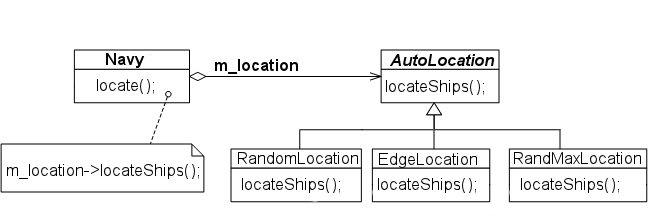
\includegraphics[scale=0.7]{locations.png}
	\caption{Схема классов паттерна ``Стратегия'' для автоматической расстановки кораблей.}
	\label{fig:location}
	\vspace{-0.5cm}
\end{center}
\end{figure}

Класс Navy представляет собой игровое поле, он включает информацию о кораблях, их местоположении и состояниях, а также предоставляет набор функций по их управлению. В качестве одного из закрытых членов используется указатель на абстрактный класс -- m\_location. При запросе расстановки кораблей вызывается функция locate(), которая в свою очередь вызывает функцию locateShips(), замещаемую в производных классах RandomLocation, RandMax-Location и EdgeLocation. Первая тактика расстановки кораблей предлагает равновероятное положение кораблей на игровом поле; вторая --  расставляет корабли, максимизируя свободное пространство; а третья -- является синтезом первых двух, она максимизирует свободное пространство при расстановке все кораблей, кроме однопалубных, а их в свою очередь равновероятно расставляет по этим свободным полям. При использовании последней тактики противник быстро найдет все многопалубные корабли, а на поиск однопалубных у него уйдет много времени.

\subsubsection{Паттерн ``Фабричный метод''}
\begin{figure}[h!]
\lstset{frame=shadowbox,label=lstfabr,caption={Фабричная функция создания объектов стратегий автоматической расстановки кораблей. Переменная ind содержит индекс элемента выпадающего списка в интерфейсе пользователя, в котором содержатся доступные стратегии.}}
\lstinputlisting{fabr.cpp}
\end{figure}
Паттерн ``фабричный метод'' -- это порождающий шаблон проектирования, который предоставляет подклассам интерфейс для создания экземпляров некоторого класса. Это позволяет использовать в коде программы не специфические классы, а манипулировать абстрактными объектами на более высоком уровне. Также известен под названием виртуальный конструктор.

В программе ``Морской бой'' определены три метода автоматического размещения кораблей с использованием шаблона проектирования ``стратегия''. Для создания конкретного экземпляра класса стратегии мы используем фабричную функцию, код которой представлен в листинге~\ref{lstfabr}. Поскольку возвращается указатель, то память с необходимостью должна быть освобождена в конце работы программы. В данной реализации за освобождение ресурсов ответственен класс Navy, в деструкторе которого помещен соответствующий оператор delete. 


\subsubsection{Паттерн ``Одиночка''}

Для многих задач требуется, чтобы некоторый класс был всегда один, и нельзя было создать дополнительные экземпляры класса. Например, в программе ``Морской бой'' изображения кораблей хорошо бы хранить в одном единственном классе и обращаться к нему по мере необходимости, получая требуемое изображение. В противном случае пришлось бы для каждого корабля хранить свою картинку, что привело бы к перерасходу памяти: на четыре однопалубных корабля пришлось бы хранить четыре одинаковые изображения. Использование паттерна ``Одиночка'' в данном случае позволяет хранить столько изображений, сколько их есть на самом деле, а не сколько клиентов их будет использовать. Аналогичную функциональность предоставляет класс QPixmapCache, однако ввиду практической важности этого паттерна был разработан соответствующий класс Singleton. 

Главная особенность классов-одиночек заключается в том, что их конструкторы представлены закрытыми функциями, поэтому создание объекта вне этого класса приводит к ошибке времени компиляции. Как правило, у таких классов есть публичная статическая функция, которая создает при необходимости объект и делегирует ему запросы клиентов. Программный код класса singleton показан в листинге \ref{lstSingle}.

\begin{figure}[t!]
\lstset{frame=shadowbox,label=lstSingle,caption={Паттерн ``Одиночка''.}}
\lstinputlisting{single.cpp}
\end{figure}

\subsection{Принцип работы сервера}

В компьютерной литературе рабочий процесс часто называют worker-ом. В соответствии с этой терминологией различают два вида серверов: использующие в качестве worker’а процесс и использующие в качестве worker’а поток. Для улучшения производительности иногда используют оба типа одновременно, порождая несколько процессов и множество потоков в каждом. У каждого процесса своё адресное пространство, что повышает надежность и отказоустойчивость системы. Однако этот способ является весьма ресурсоёмким, поэтому часто особенно для несложных сетевых служб используется многопоточная модель. Потоки, в отличие от процессов, имеют общие, разделяемые структуры данных, и на их создание операционная система тратит меньше ресурсов. В коде worker'а должна быть реализована синхронизация доступа, чтобы одновременная запись одной и той же структуры, доступной из разных параллельно выполняющихся потоков, не привела к хаосу.
\begin{figure}[t!]
\begin{center}
	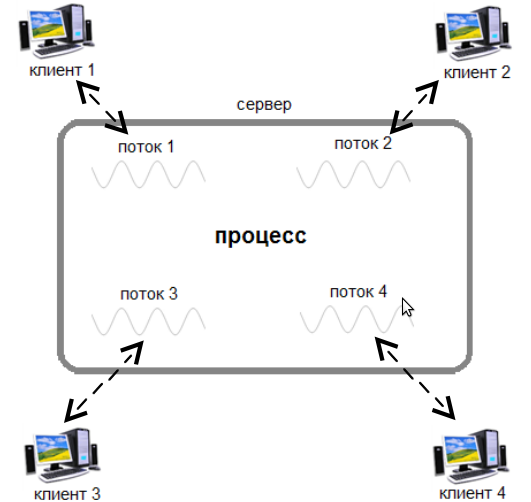
\includegraphics[scale=0.5]{threads.png}
	\caption{Схема многопоточного сервера.}
	\label{fig:threads}
        \vspace{-0.5cm}
\end{center}
\end{figure}

В нашем случае для обеспечения взаимодействия между клиентами worker’ам необходимо иметь доступ к общим данным и структурам,  поэтому в качестве основного типа worker’а был выбран поток. В результате был написан многопоточный сервер, рис. \ref{fig:threads}. Сервер написан на языке C++. Синхронизация потоков выполнена с помощью мьютексов (mutex) – особых объектов, которыми может владеть только один процесс или поток.
\begin{figure}[b!]
\begin{center}
	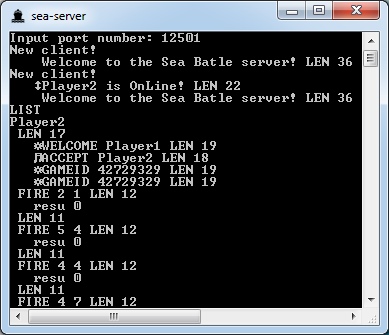
\includegraphics[scale=0.6]{server.png}
	\vspace{-.1cm}
	\caption{Скриншот консоли сервера в момент игры.}
	\label{fig:server}
        \vspace{-.8cm}
\end{center}
\end{figure}

Код сервера, отвечающий за установление клиентов, показан в листинге \ref{lstMain}. Поскольку целью работы является создание кроссплатформенного сервера, а программные интерфейсы сетевых подсистем операционных систем семейств Windows и Unix немного различаются, то устранить это различие можно при помощи условной компиляции с использованием директив препроцессора. Строки 3--9 отвечают за инициализацию, а строки 39--41 за освобождение занимаемых сетевых ресурсов сетевой подсистемы в системах Windows. 

Строки 10--20 отвечают стандартным настройкам создания сокета на стороне сервера. Бесконечный цикл, записанный в 21--38 отвечает за обработку клиентов. После поступления запроса на соединение от какого-либо клиента, создается отдельный поток, который будет его обслуживать (32-36). В качестве библиотеки по созданию и управлению потоков использовали библиотеку PThreads.

\begin{figure}[b!]
\lstset{frame=shadowbox,label=lstMain,caption={Функция main() сервера.}}
\lstinputlisting{main.cpp}
\end{figure}



Особо следует отметить строку 36. В ней происходит блокировка мьютекса. Параметр идентификатора клиента \textit{client} передаётся в потоковую функцию \textit{Child} как указатель. Может произойти такая ситуация: по каким-либо причинам потоковая функция не запустилась, а в это время \textit{accept} приняла запрос на соединение от нового клиента. В этом случае теряется идентификатор предыдущего клиента. Чтобы устранить этот эффект, была введена критическая секция, которая начинается с момента создания потока и до момента, когда потоковая функция не сохранит идентификатор своего клиента в надёжном месте, например, в свой собственной стековой переменной. При таком подходе потоковая функция всегда будет получать правильное значение номера клиента. 

В качестве параметра в потоковую функцию передается идентификатор клиента, по которому сервер взаимодействует с данным клиентом. В этой функции организован разбор приходящих от клиента сообщений и команд, список которых представлен в табл.~\ref{tbl:protocol}.

\begin{table}[t!]
\caption{Команды разработанного протокола.}
\label{tbl:protocol}
\begin{tabular}{m{3cm}m{14cm}}\toprule
Команда & Описание \\ \midrule
LOGIN & Регистрация пользователя в системе. В качестве параметра передаётся логин пользователя (ник). \\
LIST & Запрос на отображение списка всех зарегистрированных в системе пользователей. \\
SEND & Команда отправки сообщения. Первым параметром задаётся имя пользователя, а затем указывается передаваемая строка текста. \\
WELCOME & Запрос на начало игры от пользователя, передаваемого в качестве параметра. \\
ACCEPT & Одобрение запроса на начало игры. \\
REJECT & Отказ пользователя от предлагаемой игры. \\
\bottomrule
\end{tabular}
\end{table}

Если сообщение от клиента начинается не с команды, то оно трактуется как простой обмен сообщений между пользователями и передается игрокам в окне чата.

Часто серверное программное обеспечение при работе с клиентами оперирует статическими буферами для сохранения полученной от пользователя команды. Недостатком такого подхода является ошибочная обработка данных в случае поступления более длинных команд, что часто используется злоумышленниками для нарушения работы сервера. В связи с этим, в реализованном сервере активно используется динамическая память и контроль выхода за границы буферов. Максимальный размер буфера составляет 1024 байта.

\section{Искусственные нейронные сети}

Искусственные нейронные сети используются там, где трудно или практически невозможно описать в явном виде зависимость между интересующими данными. Спектр их приложений чрезвычайно широк: прогнозирование изменений на фондовой бирже, оптическое распознавание символов, диагностика состояния человека и различного рода технологических установок, автоматическое управление машинами и многое другое. Создание искусственных нейронных сетей было продиктовано попыткой понять принципы работы человеческого мозга, и хотя на сегодняшний день искусственные нейронные сети представляют весьма упрощенные от него абстракции, большинство задач получают с их помощью адекватную оценку, и сами они являются во многих областях незаменимыми помощниками человека. 

Нейронная сеть представляет собой совокупность примитивных вычислительных устройств (элементов, узлов), называемых по аналогии с биологическими системами –   нейронами, рис.~\ref{fig:neurons}. Все элементы сети связаны между собой так, чтобы между ними обеспечивалось взаимодействие. Каждый нейрон принимает и передает сигнал, преобразуя его в соответствии с некоторым правилом активации. 

\begin{figure}[t!]
\begin{center}
	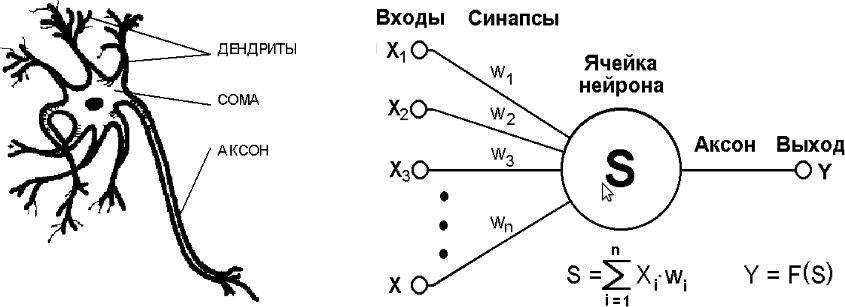
\includegraphics[scale=0.35]{neurons.png}
	\caption{Биологический нейрон слева и его математическая модель справа.}
	\label{fig:neurons}
        \vspace{-0.5cm}
\end{center}
\end{figure}

Выходной сигнал элемента может посылаться другим элементам по взвешенным связям, каждая из которых характеризуется весовым коэффициентом или весом. В зависимости от  его значения передаваемый сигнал либо усиливается, либо подавляется. 

Некоторые нейроны сети предназначены только для того, чтобы вводить информацию  из окружающей среды -- это входные элементы, аналогично определяются и выходные элементы, как нейроны, представляющие результат обработки некоторого набора данных сетью. В одной модели каждый элемент может быть связан со всеми другими элементами сети, в другой -- нейроны могут быть организованы в некоторой упорядоченной по уровням (слоям) иерархии. Возможности наложения связей на элементы сети практически бесконечны. Каждая связь характеризуется некоторыми параметрами: элементом сети, от которого эта связь исходит, элементом, к которому данная связь доставляет сигнал, ее весом, правилом учета этого веса при обработке сигнала и некоторыми другими. Рассмотрим более детально один из самых широко  распространенных типов сетей, который отвечает задачам машинного обучения с учителем.

\subsection{Многослойная сеть с прямой связью}

Пример такого рода сети представлен на рис.~\ref{fig:net}. Для простоты на нем изображено только три слоя, хотя их количество  ограничено только фантазией и опытом экспериментатора. Из теории известно, что трех слоев достаточно для аппроксимации любой непрерывной функции, но зачастую можно быстрее обучить сеть, имеющую большее количество слоев. На рис.~\ref{fig:net} сигнал распространяется по сети сверху вниз.  Это означает, что сигналы входного слоя подаются на вход нейронов промежуточного слоя, элементы которого в свою очередь порождают сигнал для нейронов выходного слоя. Входящие сигналы элементов комбинируются путем суммирования их взвешенных сумм.

Для всех элементов сети имеется правило вычисления выходного значения, которое предполагается передать другим нейронам или во внешнюю среду, если речь идёт об элементах выходного слоя. Это правило называется функцией активации. Применяются различные функции активации: тождественная – вход нейрона подаётся на выход без преобразования, пороговая – ограничивает выход значениями 0 или 1 в зависимости от некоторого порогового значения комбинированного ввода, сигмоидальная – выходные значения получаются посредством преобразования:

\begin{equation}
f(x) = {1 \over {1+exp(-x)}}
\end{equation}

\begin{wrapfigure}{r}{0.4\textwidth}
  \vspace{-0.5cm}
  \begin{center}
    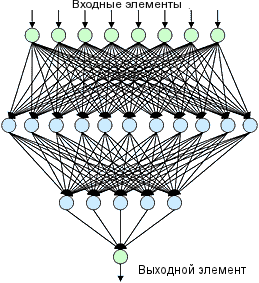
\includegraphics[scale=0.61]{net.png}
  \end{center}
  \vspace{-0.3cm}
  \caption{Трёхслойная нейронная сеть прямого распространения.}
  \label{fig:net}
  \vspace{-0.55cm}
\end{wrapfigure}Одно из главных преимуществ нейронных сетей заключается в том, что они предполагают наличие правил, с помощью которых сеть может настраиваться автоматически. Типичной формой обучения является управляемое обучение, когда для каждого набора данных, подающегося в процессе обучения на вход сети, известен соответствующий выходной набор данных, который данная сеть должна научиться прогнозировать.

Обычно в начале обучения весовые коэффициенты устанавливаются равными случайным малым значениям, так что в первый раз при предъявлении сети учебного образца оказывается весьма маловероятным, чтобы сеть произвела верный вывод. Расхождение между прогнозом сети и тем, что для данного учебного набора должно быть получено на самом деле, составляет ошибку, которая может использоваться для корректировки весов. Поэтому сам процесс обучения не что иное, как процесс адаптации весовых значений сети под конкретную задачу. В терминах машинного обучения эту задачу также называют обучение с учителем, потому что для каждого учебного набора известен желаемый результат.

\subsection{Применение искусственных нейронных сетей для выбора хода компьютера в игре ``Морской бой''}

Использование нейронной сети предполагает несколько этапов. Сначала собирается необходимый набор данных для обучения, затем на основе этой информации с использованием различных архитектур нейронных сетей и методов их обучения строится несколько наборов моделей, из которых выбираются наилучшие. Отобранные таким образом модели встраиваются в программу «Морской бой» для того, чтобы определить в какую клетку поля противника осуществить удар. Поскольку применение искусственных нейронных сетей должно приводить к повышению доли побед компьютера по сравнению с другими эвристическими алгоритмами, то интересно сравнить и количественно оценить это превышение. 

\subsubsection{Набор данных для обучения}

Для составления представительного набора данных для обучения была реализована программа «Морской бой», которая записывала в специальный файл состояние поля противника и удар, который производит человек, играя в эту игру. Такая программа была разослана через социальные сети, и около 100 человек приняли участие в тестировании. После этого все данные были объединены в один файл, примерный формат которого показан ниже:
~\newline

{\scriptsize

5052525555055555515500055551550005525055000555505500055555550000101525000555552500001055250005555555 => 2 2

0010500005050500055005550550000000000000000000000000000000000000000000000000000000000000000000000000 => 2 8

0000050552000050155500000505550000055555000000000500000000050000000005000000000500000000050000000005 => 9 8

5050500055005000555200055555550000522225005055555505000050000000000000000000500500005000005050000000 => 0 7

5552252522505555555550000000055000000005500000000550000000555000000052500000005255000000522555555555 => 1 1

5052525555055555515500005551550000525055000055505500000555550000001525000005552500000055250000055555 => 9 4

5555555525255255152555555505255550000555555000055552500005555555000555552500555525550001012510005555 => 9 5

0000000000000000000000000000000000000000000000000000000000000000000000000000000000000000000000000000 => 3 4

0000000052000000005200000000550000000001000000005500000000010000000055000000000100000000550000000000 => 9 9

5555555525255255152555555505255550000555555555055552552505555555250555552555555525555001012510555555 => 3 4

5555555555255555252555525525555552552525555255252525555555555525555222552555555555555550005255555505 => 8 7

0000000000000505000000000550000000000000000000000000000000000000000000000000000000000000000000000000 => 2 7

0000000000000000000000000000000000000000000000050500005555150000000505000000000000000000000000000000 => 3 9

2555555555552252551555555555055550000000525000000052500000005550000000525000000052500000005550000000 => 2 8

}

\vspace{0.3cm}
Слева до знака ``=>'' показано состояние поля во внутренней кодировке программы, которая учитывает состояние каждой клетки: был произведен удар, но мимо; корабль подбит; корабль убит; удара пока еще не было. Всего таких элементов 100, поэтому и размерность входного слоя нейросети будет также равна 100 нейронам. Справа же показан ход человека, который проанализировал ситуацию на вражеском поле и принял решение, руководствуясь своим опытом, тактикой и интуицией.
Всего таких векторов набралось свыше 120000. Из них были исключены дубликаты, а сами векторы были равновероятно перемешаны с использованием программы shuf. Значение каждой компоненты вектора были нормированы на отрезок [0,1].

\subsubsection{Построение нейросетевых моделей}

Построение нейросетевых моделей проводилось с помощью программы backprop \cite{backprop}. Выборка для обучения составила 108000 примеров, выборка для контроля -- 12000. Обучение нейросети прекращали, когда ошибка на примерах контрольной выборки начинала расти и превышала ошибку на тестовой на 5\%. 
Было построено 10 моделей, характеристики которых приведены в табл.~\ref{tbl:models}.
\begin{table}[h!]
\caption{Параметры построенных моделей.}
\label{tbl:models}
\begin{tabular}{>{\centering\arraybackslash}m{1cm}>{\centering\arraybackslash}m{5cm}>{\centering\arraybackslash}m{5cm}>{\centering\arraybackslash}m{5cm}}\toprule
№ & Кол-во скрытых нейронов & Ошибка обучения & Ошибка контроля \\ \midrule
1 & 8 & 8.20 & 7.81 \\
2 & 12& 6.45 & 6.14 \\
3 & 16& 6.54 & 6.23 \\
4 & 24& 6.09 & 5.79 \\
5 & 32& 5.66 & 5.39 \\
6 & 36& 5.23 & 4.98 \\ \midrule
\textbf{7}& \textbf{38}& \textbf{4.81} & \textbf{4.58} \\ \midrule
8& 40& 5.65 & 5.38 \\
9& 44& 5.06 & 4.81 \\
10& 48& 5.44 & 5.17 \\
\bottomrule
\end{tabular}
\end{table}
График зависимости ошибок на обучающей и тестовой выборок от эпохи обучения показан на рис.~\ref{fig:learning}.
\begin{figure}[h]
\begin{center}
	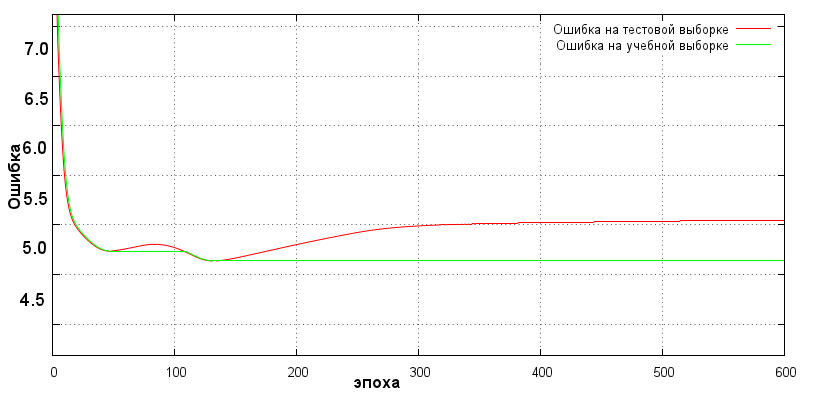
\includegraphics[scale=0.5]{learning.png}
	\caption{Зависимость ошибки прогноза от эпохи обучения.}
	\label{fig:learning}
        \vspace{-0.5cm}
\end{center}
\end{figure}
Графически зависимость эффективности моделей от количества скрытых нейронов показана на рис.~\ref{fig:effectiveness}. 
\begin{figure}[t!]
\begin{center}
	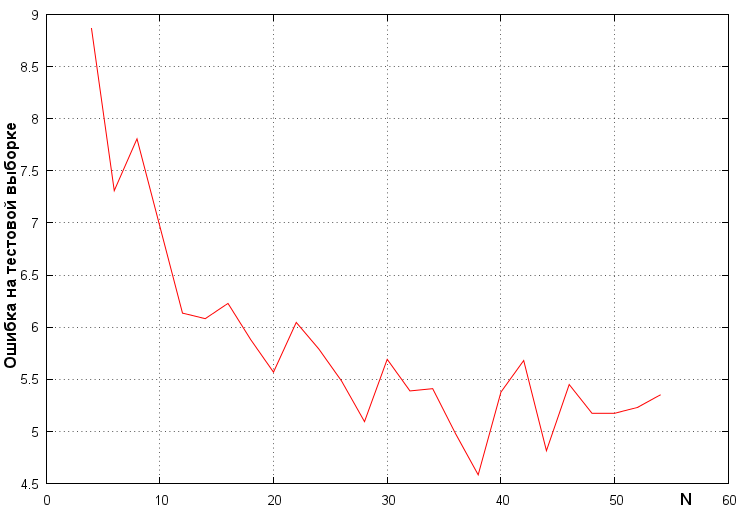
\includegraphics[scale=0.5]{effectiveness.png}
	\caption{Зависимость ошибки прогнозирования модели на тестовой выборке от количества скрытых нейронов.}
	\label{fig:effectiveness}
        \vspace{-0.5cm}
\end{center}
\end{figure}

Наилучшая модель характеризуется ошибкой $\le 5$, поэтому она была интегрирована в программу ``Морской бой''.

\subsubsection{Оценка эффективности нейросетевого подхода}

Для оценки эффективность нейросетевого подхода был проведен численный эксперимент. Компьютер играл против компьютера (сам с собой) в течение 100000 партий в «Морской бой». Сначала для оценки правильности разработанного нами алгоритма (решателя) мы проверили результаты поединка с использованием только равновероятного подхода. Этот алгоритм близок стратегии, с помощью которой играет человек. Если на поле противника существует подбитый корабль, то необходимо его потопить и только после этого переходить к поиску следующих кораблей, который основан на равновероятном выборе поля, где бы мог находиться корабль. Очевидно, что при большом количестве игр, результат поединка должен быть равным. Это подтвердилось нашим компьютерным экспериментом. Из 100000 партий первый решатель выиграл 49859 игр, а второй — 50141. Расхождение между ними составляет меньше 1\%. 

Убедившись, что наша система работает правильно и не противоречит законам математики, мы изменили первый решатель таким образом, чтобы искусственная нейронная сеть предлагала вариант удара вместо равновероятного выбора. Однако поскольку нейросеть может ошибиться, то мы реализовали проверку, что если выход нейросети попадает в уже исследованную клетку поля или вообще вне поля, то используется как и в первом случае равновероятный выбор из свободных клеток. Таким образом, было проведено 100000 партий между искусственной нейронной сетью и обычным решателем. Результаты таковы: нейросеть выиграла 60515 игры, а обычный алгоритм – 39485. Расхождение составляет 21030 партий. А общий выигрыш превышает 21\%. 

\section{Платформа игрового сервера}

Разработанный игровой сервер ``Морской бой'' размещен по адресу \url{31.31.201.23} по порту 12501. Технические характеристики сервера 500 MHz CPU, 256 MB RAM, 5 GB HDD. Сервер находится под управлением операционной системы OpenSuse 11.1.
\newpage

\section*{Выводы}
\addcontentsline{toc}{section}{Выводы}

В результате работы был создан платформонезависимый многопоточный сервер для координации игроков игры ``Морской бой'', который также может работать в режиме чата. Также было разработано графическое приложение-клиент для этой сетевой игры. На основе данных реальных игровых партий были построены нейросетевые модели и показана эффективность их применения по сравнению с обычным равновероятным поиском.

\nocite{maks}
\nocite{zemskov}
\nocite{Callan}
\nocite{backprop}
\nocite{Haykin}

\newpage
\bibliography{biblio}
\bibliographystyle{gost705}

\end{document}
